\documentclass[aspectratio=169,10pt]{beamer}

\usetheme{Madrid}
\usecolortheme{seahorse}
\usepackage{amsmath, amssymb, amsfonts}
\usepackage{mathtools}
\usepackage{listings}
\usepackage{xcolor}
\usepackage{tikz}
\usetikzlibrary{arrows, shapes, positioning}

% Set up graphics path
\graphicspath{{figures/}}

% Custom colors
\definecolor{darkblue}{RGB}{0, 51, 102}
\definecolor{darkgreen}{RGB}{34, 139, 34}
\definecolor{darkred}{RGB}{139, 0, 0}

% Listings setup for code
\lstset{
    basicstyle=\ttfamily\scriptsize,
    keywordstyle=\color{blue},
    commentstyle=\color{green!50!black}\itshape,
    stringstyle=\color{red},
    breaklines=true,
    numbers=left,
    numberstyle=\tiny,
    frame=single,
    language=Python
}

% Footer
\setbeamertemplate{footline}[frame number]

% Theorem environments
\newtheorem{proposition}[theorem]{Proposition}
\newtheorem{corollary}[theorem]{Corollary}

\title{Fixed Point Theorems}
\subtitle{Chapter 5: Brouwer, Schauder, and Beyond}
\author{Based on Pathak's Introduction to Nonlinear Analysis (2018)}
\date{}

\begin{document}

% ============================================================================
% TITLE SLIDE
% ============================================================================
\frame{\titlepage}

% ============================================================================
% TABLE OF CONTENTS
% ============================================================================
\begin{frame}[allowframebreaks]{Outline}
\tableofcontents
\end{frame}

% ============================================================================
% SECTION 1: INTRODUCTION AND BASIC CONCEPTS
% ============================================================================
\section{Foundations: Nonexpansive and Asymptotically Nonexpansive Mappings}

\begin{frame}[allowframebreaks]{Nonexpansive Mappings: Overview}
    \begin{definition}
        A mapping $T: K \to K$ on a nonempty subset $K$ of a normed linear space $X$ is said to be:
        \begin{enumerate}
            \item \textbf{Nonexpansive} if $\|Tx - Ty\| \le \|x - y\|$ for all $x,y \in K$
            \item \textbf{Contractive} if $\|Tx - Ty\| \le \alpha\|x - y\|$ for some $0 < \alpha < 1$
        \end{enumerate}
    \end{definition}

    \begin{block}{Key Observation}
        Banach's contraction principle guarantees unique fixed points for contractive mappings, but nonexpansive mappings may not have fixed points without additional assumptions.
    \end{block}

    \begin{example}[Nonexpansive Without FPP]
        On the unit circle $S^1 = \{x \in \mathbb{R}^2: \|x\| = 1\}$, a rotation by angle $\theta \neq 2\pi k$ is nonexpansive but has no fixed point.
    \end{example}
\end{frame}

\begin{frame}[allowframebreaks]{Pseudocontractive Mappings}
    \begin{definition}[Definition 5.23]
        Let $K$ be a nonempty subset of a normed linear space $X$. A mapping $F: K \to X$ is said to be \textbf{pseudocontractive} if for each $k > 0$ and for all $x, y \in K$:
        \[
        \|x - y\| \le \|(1 + k)(x - y) - k(Fx - Fy)\|
        \]
    \end{definition}

    \begin{block}{Hilbert Space Characterization}
        In a real Hilbert space with corresponding norm, this is equivalent to:
        \[
        (Fx - Fy, x - y) \le \|x - y\|^2 \quad \text{for all } x, y \in K
        \]
    \end{block}

    \begin{block}{Connection to Accretive Operators}
        Pseudocontractive mappings are closely related to accretive operators through the relationship:
        \[
        T = I - F \text{ is accretive} \iff F \text{ is pseudocontractive}
        \]
    \end{block}
\end{frame}

% ============================================================================
% SECTION 2: ASYMPTOTICALLY NONEXPANSIVE MAPPINGS
% ============================================================================
\section{Asymptotically Nonexpansive Mappings and Weak Convergence}

\begin{frame}[allowframebreaks]{Asymptotically Nonexpansive Mappings}
    \begin{definition}[Definition 5.24]
        Let $K$ be a nonempty subset of a Banach space $X$. A mapping $T: K \to K$ is said to be \textbf{asymptotically nonexpansive} if:
        \[
        \|T^n x - T^n y\| \le k_n \|x - y\| \quad \text{for all } x, y \in K \quad \text{and} \quad \lim_{n \to \infty} k_n = 1
        \]
    \end{definition}

    \begin{block}{Key Properties}
        \begin{itemize}
            \item More general than nonexpansive mappings
            \item Sequence of constants $\{k_n\}$ approaches 1
            \item Not all asymptotically nonexpansive mappings are nonexpansive
        \end{itemize}
    \end{block}

    \begin{block}{Historical Note}
        Goebel and Kirk proved fundamental theorems for this class in 1972, extending Banach's theory to this more general setting.
    \end{block}
\end{frame}

\begin{frame}[allowframebreaks]{Asymptotic Regularity}
    \begin{definition}[Definition 5.25]
        A mapping $T: K \to K$ is said to be \textbf{asymptotically regular} if for any $x \in K$:
        \[
        \|T^n x - T^{n+1} x\| \to 0 \quad \text{as } n \to \infty
        \]
    \end{definition}

    \begin{block}{Significance}
        Asymptotic regularity is a weaker condition than having a fixed point, yet it provides crucial control over the iterative behavior of the mapping.
    \end{block}

    \begin{theorem}[Bose, 1970]
        Let $X$ be a uniformly convex Banach space with weakly continuous duality mapping and $K$ a nonempty, bounded, closed and convex subset of $X$. If $T: K \to K$ is asymptotically nonexpansive and asymptotically regular, then for any $x \in K$, the sequence $\{T^n x\}$ converges weakly to a fixed point of $T$.
    \end{theorem}
\end{frame}

\begin{frame}[allowframebreaks]{Opial's Condition}
    \begin{definition}[Definition 5.26]
        A Banach space $X$ is said to satisfy \textbf{Opial's condition} if for each $x_0 \in X$ and each sequence $\{x_n\}$ weakly converging to $x_0$, the inequality:
        \[
        \liminf_{n \to \infty} \|x_n - x\| > \liminf_{n \to \infty} \|x_n - x_0\|
        \]
        holds for all $x \neq x_0$.
    \end{definition}

    \begin{block}{Equivalent Form (Weak Opial's Condition)}
        If a sequence $\{x_n\}$ is weakly convergent to $x_0$ in $X$, then for every $x \in X$:
        \[
        \limsup_{n \to \infty} \|x_n - x\| \ge \limsup_{n \to \infty} \|x_n - x_0\|
        \]
    \end{block}

    \begin{observation}
        \begin{itemize}
            \item Every Hilbert space and $\ell_p$ spaces ($1 < p < \infty$) satisfy Opial's condition
            \item Banach spaces with weakly continuous duality mappings satisfy weak Opial's condition
            \item Opial proved this inequality is strict for $x \neq x_0$
        \end{itemize}
    \end{observation}
\end{frame}

\begin{frame}[allowframebreaks]{Convergence Theorem for Asymptotically Nonexpansive Maps}
    \begin{theorem}[Theorem 5.43 - Bose, 1971]
        Let $X$ be a uniformly convex Banach space having weakly continuous duality mapping and $K$ a nonempty, bounded, closed and convex subset of $X$. Suppose $T: K \to K$ is asymptotically nonexpansive and asymptotically regular. Then for any $x \in K$, the sequence $\{T^n x\}$ converges weakly to a fixed point of $T$.
    \end{theorem}

    \begin{block}{Proof Outline}
        \begin{enumerate}
            \item Every weak cluster point of $\{T^n x\}$ is a fixed point (by asymptotic regularity)
            \item Opial's condition ensures all weak cluster points coincide
            \item Uniform convexity provides the convergence framework
        \end{enumerate}
    \end{block}

    \begin{corollary}[Corollary 5.12]
        Let $K$ be a closed, convex and bounded subset of $X$ and let $T: K \to K$ be weakly continuous and asymptotically nonexpansive. If $T$ is asymptotically regular at $x_0 \in K$, then $\{T^n x_0\}$ converges weakly to a fixed point of $T$.
    \end{corollary}
\end{frame}

\begin{frame}[allowframebreaks]{Sequences of Asymptotically Nonexpansive Mappings}
    \begin{definition}[Definition 5.27]
        The sequence $\{T_n\}$ of self-mappings of $K$ is said to be \textbf{asymptotically nonexpansive} if:
        \[
        \|T_n x - T_n y\| \le k_n \|x - y\| \quad \text{for all } x, y \in K \quad \text{with} \quad \lim_{n \to \infty} k_n = 1
        \]
    \end{definition}

    \begin{block}{Fixed Point Set Notation}
        We denote the set of fixed points of mapping $T$ by $\mathcal{F}(T) = \{x \in K: Tx = x\}$.
    \end{block}

    \begin{theorem}[Theorem 5.44 - Pasty, extending Opial]
        Let $X$ be a uniformly convex Banach space with Fréchet differentiable norm and $K$ a closed and convex subset of $X$. Let $C$ be a subset of $K$ and $S = \{T_n\}_{n=1}^{\infty}$ an asymptotically nonexpansive sequence of self-mappings of $K$ such that:
        \begin{enumerate}
            \item $C \subset \bigcap_{n=1}^{\infty} \mathcal{F}(T_n)$
            \item There exists $x_0 \in K$ for which $T_n x_0 \to z$ implies $z \in C$
            \item $T_n T_m x_0 - T_n x_0 \to 0$ as $n \to \infty$ for all fixed $m$
        \end{enumerate}
        Then either $C = \emptyset$ and $\|T_n x_0\| \to +\infty$, or $C \neq \emptyset$ and $T_n x_0$ converges weakly to an element of $C$.
    \end{theorem}
\end{frame}

% ============================================================================
% SECTION 3: BROUWER AND SCHAUDER THEOREMS
% ============================================================================
\section{Classical Fixed Point Theorems: Brouwer and Schauder}

\begin{frame}[allowframebreaks]{The Fixed Point Property}
    \begin{definition}[Definition 5.28]
        A topological space $X$ is said to possess the \textbf{fixed point property} (FPP) if every continuous function of $X$ into itself has a fixed point.
    \end{definition}

    \begin{block}{Examples with FPP}
        \begin{itemize}
            \item Closed unit interval $[0, 1]$ in $\mathbb{R}$
            \item Finite closed interval $[a, b]$
            \item Closed unit disk in the plane
        \end{itemize}
    \end{block}

    \begin{block}{Important Remarks}
        \begin{itemize}
            \item It is difficult to establish FPP in general settings
            \item FPP is preserved under homeomorphisms (Theorem 5.45)
            \item Retracts play a crucial role in FPP theory
        \end{itemize}
    \end{block}
\end{frame}

\begin{frame}[allowframebreaks]{Partition of Unity}
    \begin{definition}[Definition 5.29]
        Suppose $V_1, \ldots, V_n$ are open subsets of a locally compact Hausdorff space $X$, $K \subset X$ is compact, and:
        \[
        K \subset V_1 \cup \cdots \cup V_n
        \]
        Then for every $j = 1, \ldots, n$ there exists $\varphi_j \in C(X)$, with $0 \le \varphi_j \le 1$, supported on $V_j$ such that:
        \[
        \varphi_1(x) + \cdots + \varphi_n(x) = 1, \quad \forall x \in K
        \]
        The collection $\{\varphi_1, \ldots, \varphi_n\}$ is called a \textbf{partition of the unity} for $K$ subordinate to the open cover $\{V_1, \ldots, V_n\}$.
    \end{definition}

    \begin{block}{Connection to Functional Analysis}
        The partition of unity is fundamental in constructing continuous functions and proving existence results in functional analysis.
    \end{block}
\end{frame}

\begin{frame}[allowframebreaks]{Retracts and the Fixed Point Property}
    \begin{theorem}[Theorem 5.46]
        Any nonempty, closed and convex subset $K$ of $\mathbb{R}^n$ or of a Hilbert space or of a Banach space $X$ is a retract of any larger subset.
    \end{theorem}

    \begin{theorem}[Theorem 5.47]
        If $Y$ has the fixed point property and $X$ is a retract of $Y$, then $X$ has the fixed point property.
    \end{theorem}

    \begin{block}{Proof Strategy}
        Let $R$ be a retraction of $Y$ onto $X$. If $F: X \to X$ is continuous, then $FR: Y \to X \subset Y$ is continuous. By FPP of $Y$, there exists $u \in Y$ such that $FRu = u$. If $u \in X$, then $Fu = u$. If $u \notin X$, we reach a contradiction.
    \end{block}

    \begin{block}{Remark}
        These results are foundational for proving Brouwer's and Schauder's theorems using retraction arguments.
    \end{block}
\end{frame}

\begin{frame}[allowframebreaks]{Brouwer's Fixed Point Theorem}
    \begin{theorem}[Theorem 5.48 - Brouwer's FPT]
        The closed unit ball $\mathbb{B}^n$ of $\mathbb{R}^n$ has the fixed point property. Equivalently: \\
        Let $f: \mathbb{B}^n \to \mathbb{B}^n$ be a continuous function. Then $f$ has a fixed point $\bar{x} \in \mathbb{B}^n$.
    \end{theorem}

    \begin{block}{Proof Technique: Differential Forms}
        Using the theory of differential forms and Stokes' theorem:
        \begin{itemize}
            \item Assume $f$ has no fixed point
            \item Construct a continuous retraction $r: \mathbb{B}^n \to \mathbb{S}^{n-1}$ of class $C^2$
            \item Compute $\det(J_r(x)) = 0$ for all $x$, leading to a contradiction
        \end{itemize}
    \end{block}

    \begin{block}{Topological Proof}
        Alternative approach using topological degree and homology:
        \begin{itemize}
            \item Show that $\mathbb{S}^{n-1}$ is not a retract of $\mathbb{B}^n$ (topologically)
            \item Use homology to establish the contradiction
        \end{itemize}
    \end{block}
\end{frame}

\begin{frame}[allowframebreaks]{Extensions of Brouwer's Theorem}
    \begin{theorem}[Theorem 5.49]
        Every nonempty, compact and convex subset $K$ of $K$ of $\mathbb{R}^n$ (a finite dimensional normed linear space) has the fixed point property.
    \end{theorem}

    \begin{proof}
        For $r$ sufficiently large, the ball $B_r$ of radius $r$ contains $K$. By Theorem 5.46, $K$ is a retract of $B_r$. Since $B_r$ is homeomorphic to $\mathbb{B}^n$, by Theorem 5.45, $B_r$ has the FPP. Therefore, by Theorem 5.47, $K$ has the FPP.
    \end{proof}

    \begin{theorem}[Theorem 5.50]
        Brouwer's FPT is equivalent to: there exists no retraction of $\mathbb{B}^n$ onto to the boundary $\partial\mathbb{B}^n$ which is continuously differentiable.
    \end{theorem}

    \begin{theorem}[Theorem 5.51 - Consequence of Brouwer]
        Let $F: \mathbb{B}^n \to \mathbb{R}^n$ be a continuous mapping and suppose that for some $r > 0$ and all $\eta > 0$:
        \[
        F(x) + \eta x \neq 0 \quad \text{for any } x \text{ with } \|x\| = r
        \]
        Then there exists a point $x_0$, $\|x_0\| \le r$ such that $F(x_0) = 0$.
    \end{theorem}
\end{frame}

\begin{frame}[allowframebreaks]{Schauder's Fixed Point Theorem}
    \begin{theorem}[Theorem 5.55 - Schauder's FPT]
        Let $K$ be a nonempty, closed and convex subset of a normed linear space $X$. Let $T$ be a continuous mapping of $K$ into a compact subset of $K$. Then $T$ has a fixed point in $K$.
    \end{theorem}

    \begin{block}{Key Assumption}
        Unlike Brouwer, Schauder doesn't require finite dimensionality. Instead, the compactness of $T(K)$ provides the essential structure.
    \end{block}

    \begin{proof}[Proof Strategy]
        \begin{enumerate}
            \item Let $A$ be the compact subset with $T(K) \subset A \subset K$
            \item A is contained in a closed, convex, bounded subset $B$ of $X$
            \item $T(B \cap K) \subset A \subset B$, which is compact
            \item Use Brouwer's theorem on finite-dimensional approximations
            \item Extract convergent subsequences from $A$'s compactness
        \end{enumerate}
    \end{proof}
\end{frame}

\begin{frame}[allowframebreaks]{Schauder's Theorem: Extensions and Consequences}
    \begin{theorem}[Theorem 5.56]
        Let $K$ be a nonempty, compact and convex subset of a normed linear space $X$ and let $T$ be a continuous mapping of $K$ into itself. Then $T$ has a fixed point in $K$.
    \end{theorem}

    \begin{theorem}[Theorem 5.57]
        Let $T$ be a compact and continuous mapping of a normed linear space $X$ into itself and let $T(X)$ be bounded. Then $T$ has a fixed point.
    \end{theorem}

    \begin{theorem}[Theorem 5.58]
        Let $X$ be a reflexive Banach space, $K$ a closed and convex subset of $X$ and $T$ a weakly continuous mapping of $K$ into a bounded subset of $K$. Then $T$ has a fixed point $K$.
    \end{theorem}

    \begin{block}{Practical Implications}
        These extensions allow application to infinite-dimensional spaces when:
        \begin{itemize}
            \item The mapping is compact
            \item The space is reflexive with weak continuity
            \item The image has suitable boundedness properties
        \end{itemize}
    \end{block}
\end{frame}

% ============================================================================
% SECTION 4: ADVANCED FIXED POINT THEOREMS
% ============================================================================
\section{Advanced Theorems and Special Cases}

\begin{frame}[allowframebreaks]{Relative Compactness Condition}
    \begin{theorem}[Theorem 5.59]
        Let $X$ be a normed linear space. Suppose that $K$ is a nonempty, closed, and convex subset of $X$, and $T$ a continuous mapping of $K$ into itself such that $T(K)$ is relatively compact in $X$. Then $T$ has a fixed point.
    \end{theorem}

    \begin{proof}
        Let $B$ be the convex hull of $T(K)$ in $X$, and let $S$ be the closure of $B$ in $X$. Then $S \subset K$ is:
        \begin{itemize}
            \item Nonempty and convex
            \item Compact (since $T(K)$ is relatively compact)
            \item Contains $T(K)$: $T(S) = T(\overline{B}) = T(\bar{B} \cap K) \subset \overline{T(K)} = S$
        \end{itemize}
        By Theorem 5.56, $T|_S$ has a fixed point.
    \end{proof}
\end{frame}

\begin{frame}[allowframebreaks]{Krasnoselski's Fixed Point Theorem}
    \begin{theorem}[Theorem 5.61 - Krasnoselski]
        Let $K$ be a nonempty, complete and convex subset of a normed linear space $X$. Let $T$ be a continuous mapping of $K$ into a compact subset of $X$. Let $S: K \to X$ be a contradiction mapping with Lipschitz constant $\alpha$ and let $Tx + Sy \in K$ for all $x, y \in K$ for all $x, y \in K$. Then there is a point $u \in K$ such that $Tu + Su = u$.
    \end{theorem}

    \begin{block}{Key Insight}
        This theorem combines:
        \begin{itemize}
            \item Compactness of one mapping ($T$)
            \item Contractiveness of another mapping ($S$)
            \item A closure property ($Tx + Sy \in K$)
        \end{itemize}
    \end{block}

    \begin{proof}[Proof Idea]
        Define $F(x,y) = Tx + Sy$ on $K \times K$. For fixed $x$, the map $y \mapsto F(x,y)$ is a contraction. Show that the mapping $A$ defined through this process has a fixed point by Schauder's theorem.
    \end{proof}
\end{frame}

\begin{frame}[allowframebreaks]{Krasnoselski's Approximation Scheme}
    \begin{theorem}[Theorem 5.62 - Krasnoselski Approximation]
        Let $K$ be a bounded, closed and convex subset of a uniformly convex Banach space $X$. Let $T$ be a nonexpansive mapping of $K$ into a compact subset of $K$. Let $x_0$ be an arbitrary point of $K$. Then the sequence defined by:
        \[
        x_{n+1} = \frac{1}{2}(x_n + Tx_n), \quad n = 0, 1, 2, \ldots
        \]
        converges to a fixed point of $T$ in $K$.
    \end{theorem}

    \begin{block}{Practical Algorithm}
        This provides a constructive method for finding fixed points:
        \begin{enumerate}
            \item Start with arbitrary $x_0 \in K$
            \item Compute $x_{n+1} = \tfrac{1}{2}(x_n + Tx_n)$
            \item Sequence converges to a fixed point
        \end{enumerate}
    \end{block}

    \begin{proof}[Convergence Proof]
        \begin{itemize}
            \item Show $\|x_{n+1} - y\| \le \|x_n - y\|$ for any fixed point $y$
            \item Use uniform convexity and compactness
            \item Extract convergent subsequence
        \end{itemize}
    \end{proof}
\end{frame}

\begin{frame}[allowframebreaks]{Boundary Condition Theorems}
    \begin{theorem}[Theorem 5.63 - Altman's Theorem]
        Let $X$ be a normed linear space. Let $T$ be a continuous mapping of $B_r = \{x: \|x\| \le r\}$ into a compact subset of $X$ such that:
        \[
        \|Tx - x\|^2 \ge \|Tx\|^2 - \|x\|^2, \quad \text{for all } x \text{ such that } \|x\| = r
        \]
        Then $T$ has a fixed point in $B_r$.
    \end{theorem}

    \begin{theorem}[Theorem 5.64 - Rothe's Theorem]
        Let $X$ be a normed linear space and $T$ be a continuous mapping of $B_r$ into a compact subset of $X$ such that:
        \[
        T(\partial B_r) \subset B_r, \quad \text{i.e., } \|Tx\| < \|x\| \quad \forall x \in \partial B_r
        \]
        Then $T$ has a fixed point.
    \end{theorem}

    \begin{block}{Key Difference}
        Rothe's condition is more restrictive (strict inequality) but easier to verify in practice than Altman's condition.
    \end{block}
\end{frame}

\begin{frame}[allowframebreaks]{Potter's Fixed Point Theorem}
    \begin{theorem}[Theorem 5.65 - Potter's Theorem]
        Let $X$ be a normed linear space. Let $K$ be any closed and convex subset of $X$ and $T$ be a continuous mapping of $K$ into a compact subset of $X$ such that:
        \[
        T(\partial K) \subset K
        \]
        Then $T$ has a fixed point.
    \end{theorem}

    \begin{proof}[Proof Sketch]
        Define radial retraction $R$ of $X$ onto $K$ by:
        \[
        Rx = \frac{x}{\max(1, \rho(x))}
        \]
        where $\rho(x) = \inf\{\alpha: x \in \alpha K\}$ is the Minkowski functional. Then:
        \begin{itemize}
            \item $R$ is a continuous retraction
            \item $RT$ maps $K$ continuously into a compact subset of $K$
            \item By Schauder's theorem, $RT$ has a fixed point $u$
            \item This fixed point is also a fixed point of $T$
        \end{itemize}
    \end{proof}
\end{frame}

% ============================================================================
% SECTION 5: SCHAUDER-TYCHONOFF THEOREM
% ============================================================================
\section{Schauder-Tychonoff Theorem and General Topological Spaces}

\begin{frame}[allowframebreaks]{Finite-Dimensional Reduction}
    \begin{lemma}[Lemma 5.8]
        Let $K$ be a nonempty, compact and convex subset of a finite dimensional real Banach space $X$. Then every continuous function $f: K \to K$ has a fixed point $\bar{x} \in K$.
    \end{lemma}

    \begin{proof}[Proof Outline]
        Without loss of generality, assume $X$ is homeomorphic to $\mathbb{R}^n$. We can assume $K \subset \mathbb{R}^n$.
        \begin{enumerate}
            \item Let $p(x) \in K$ be the unique point of minimum norm from $x$ to $K$
            \item Define $g(x) = f(p(x))$
            \item $g$ maps $\mathbb{R}^n$ continuously onto $K$
            \item By Brouwer's theorem on finite dimensions, $g(\bar{x}) = \bar{x} = f(\bar{x})$
        \end{enumerate}
    \end{proof}

    \begin{block}{Remark}[Remark 5.25]
        If there is a compact and convex set $K \subset \mathbb{R}^n$ such that $h(K) \subset K$, then $h$ has a fixed point $\bar{x} \in K$.
    \end{block}
\end{frame}

\begin{frame}[allowframebreaks]{Schauder-Tychonoff Fixed Point Theorem}
    \begin{theorem}[Theorem 5.66 - Schauder-Tychonoff]
        Let $X$ be a locally convex space, $K \subset X$ nonempty and convex, $K_0 \subset K$ compact. Given a continuous map $f: K \to K_0$, there exists $\bar{x} \in K_0$ such that $f(\bar{x}) = \bar{x}$.
    \end{theorem}

    \begin{block}{Proof Strategy}
        \begin{enumerate}
            \item Use partitions of unity to approximate $f$ by finite-dimensional mappings
            \item For each partition $\{V_1, \ldots, V_n\}$ of $K_0$, define:
                \[f_U(x) = \sum_{j=1}^n \varphi_j(f(x)) x_j\]
                where $x_j$ are representative points
            \item Apply Brouwer's theorem on finite-dimensional convex hull
            \item Extract convergent subsequence using compactness of $K_0$
        \end{enumerate}
    \end{block}

    \begin{block}{Remark}
        This is the most general fixed point theorem in the Brouwer-Schauder family, applicable to locally convex topological vector spaces.
    \end{block}
\end{frame}

% ============================================================================
% SECTION 6: NUMERICAL METHODS AND COMPUTATIONAL ASPECTS
% ============================================================================
\section{Computational Methods and Numerical Examples}

\begin{frame}[fragile]{Mann Iteration Algorithm}
    \begin{block}{Mann Iteration Scheme}
        For a nonexpansive (or asymptotically nonexpansive) mapping $T$ on convex set $K$:
        \[
        x_{n+1} = (1 - \lambda_n) x_n + \lambda_n T(x_n), \quad n = 0, 1, 2, \ldots
        \]
        where $\{\lambda_n\}$ is a sequence with $0 < \lambda_n < 1$ and $\sum \lambda_n(1-\lambda_n) = \infty$.
    \end{block}

    \begin{lstlisting}
# Python: Mann Iteration Example
import numpy as np
import matplotlib.pyplot as plt

def mann_iteration(T, x0, lam, max_iter=100):
    """Mann iteration for fixed point computation"""
    x = np.copy(x0)
    trajectory = [x.copy()]

    for n in range(max_iter):
        Tx = T(x)
        x = (1 - lam) * x + lam * Tx
        trajectory.append(x.copy())

    return np.array(trajectory)

# Example: T(x) = 0.7*x + 0.5
T = lambda x: 0.7 * x + 0.5
x0 = 0.0

# Convergence for different lambda values
for lam in [0.3, 0.5, 0.8, 1.0]:
    traj = mann_iteration(T, x0, lam)
    print(f"λ={lam}: Limit ≈ {traj[-1]:.6f}")
    \end{lstlisting}
\end{frame}

\begin{frame}[fragile]{Krasnoselski Iteration Example}
    \begin{block}{Krasnoselski Method}
        For nonexpansive mapping $T$ on convex set $K$:
        \[
        x_{n+1} = \frac{1}{2}(x_n + Tx_n), \quad n = 0, 1, 2, \ldots
        \]
        This is Mann iteration with $\lambda_n = 1/2$.
    \end{block}

    \begin{lstlisting}
# Python: Krasnoselski Iteration Implementation
def krasnoselski_iteration(T, x0, max_iter=100, tol=1e-8):
    """Krasnoselski iteration (Mann with λ=0.5)"""
    x = np.copy(x0)
    errors = []

    for n in range(max_iter):
        Tx = T(x)
        x_new = 0.5 * (x + Tx)
        error = np.linalg.norm(x_new - x)
        errors.append(error)

        if error < tol:
            print(f"Converged in {n+1} iterations")
            break

        x = x_new

    return x, np.array(errors)

# Example on unit disk
def T_example(x):
    """Example mapping: rotation scaled"""
    theta = np.pi / 6
    rotation = np.array([[np.cos(theta), -np.sin(theta)],
                        [np.sin(theta), np.cos(theta)]])
    return 0.8 * rotation @ x

x0 = np.array([1.0, 0.0])
x_fixed, errors = krasnoselski_iteration(T_example, x0)
print(f"Fixed point: {x_fixed}")
    \end{lstlisting}
\end{frame}

\begin{frame}{Convergence Behavior Visualization}
    \begin{center}
        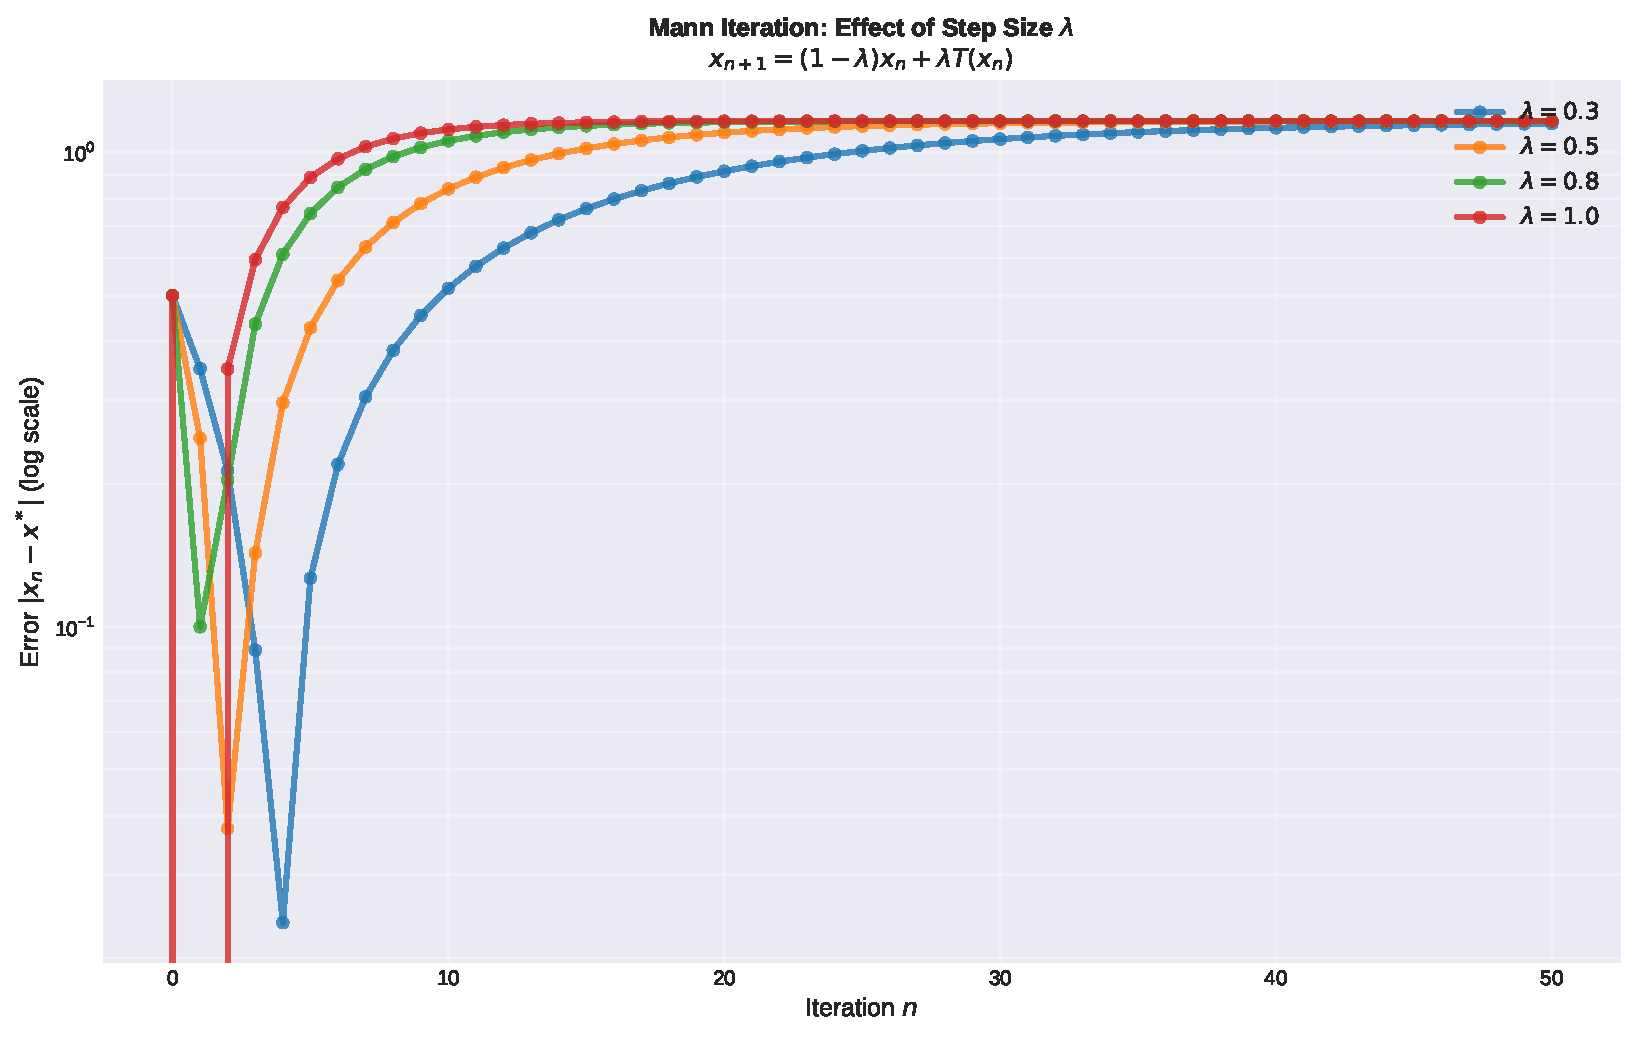
\includegraphics[width=0.9\textwidth]{mann_iteration.pdf}
    \end{center}

    \begin{block}{Key Observations}
        \begin{itemize}
            \item Standard Picard iteration ($\lambda = 1.0$) may diverge for certain mappings
            \item Lower $\lambda$ values provide more stability
            \item Optimal choice depends on the spectral properties of $T$
            \item For contractions, $\lambda = 1.0$ is optimal; for nonexpansive, smaller values help
        \end{itemize}
    \end{block}
\end{frame}

% ============================================================================
% SECTION 7: SUMMARY AND COMPARISONS
% ============================================================================
\section{Summary and Comparative Analysis}

\begin{frame}[allowframebreaks]{Mapping Hierarchy}
    \begin{center}
        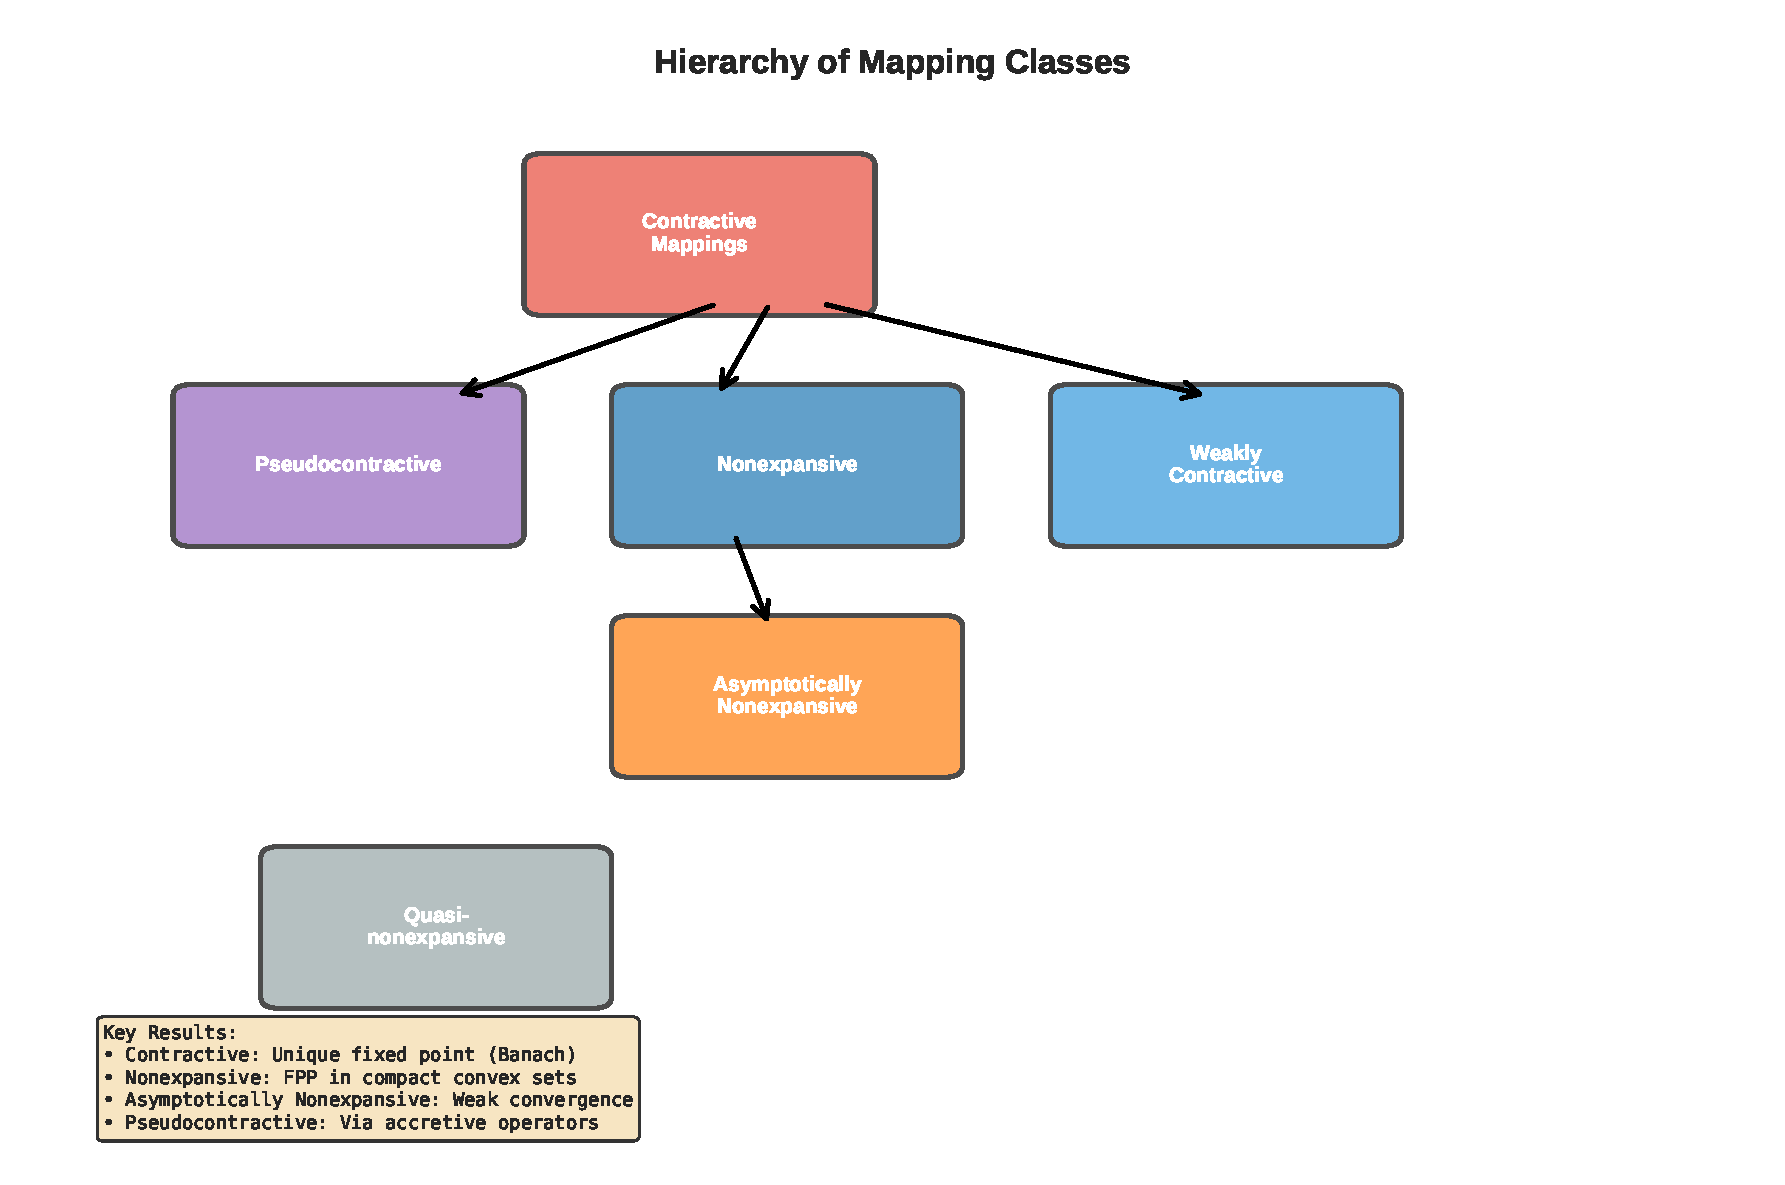
\includegraphics[width=0.95\textwidth]{mapping_hierarchy.pdf}
    \end{center}

    \begin{block}{Key Relationships}
        Contractive $\subsetneq$ Nonexpansive $\subsetneq$ Asymptotically Nonexpansive

        All imply existence of fixed points under appropriate domain conditions.
    \end{block}
\end{frame}

\begin{frame}[allowframebreaks]{Fixed Point Spaces and Results}
    \begin{center}
        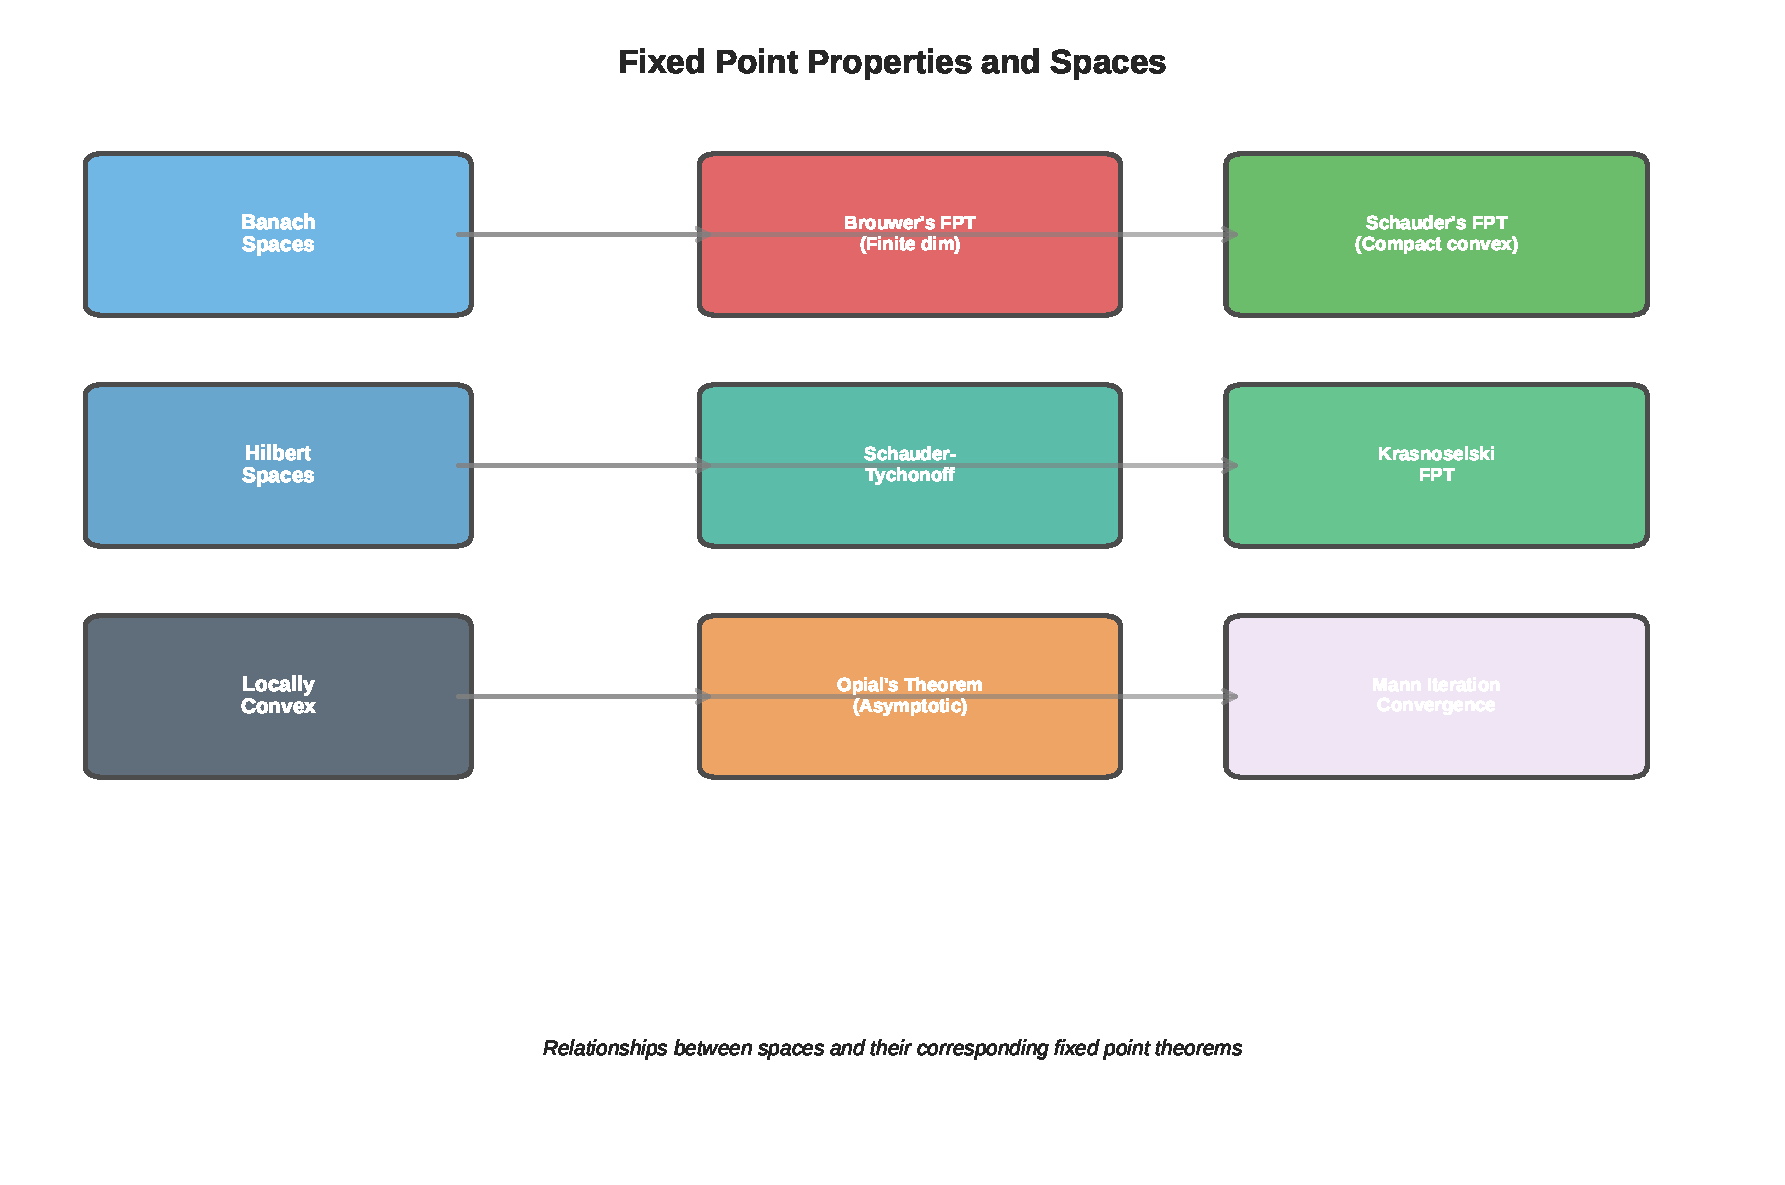
\includegraphics[width=0.95\textwidth]{fpt_properties.pdf}
    \end{center}

    \begin{block}{Domain and Mapping Combinations}
        Different space structures ($\mathbb{B}^n$, Hilbert, Banach, locally convex) combined with mapping properties (compact, continuous, weakly continuous) yield different fixed point results.
    \end{block}
\end{frame}

\begin{frame}[allowframebreaks]{Theorem Conditions Summary}
    \begin{center}
        
\includegraphics[width=1.0\textwidth]{theorem_conditions.pdf}
    \end{center}

    \begin{block}{Selection Guide}
        \begin{itemize}
            \item Finite dimensions + continuous map: Brouwer
            \item Compact map on closed convex set: Schauder
            \item Locally convex space: Schauder-Tychonoff
            \item Asymptotically nonexpansive: Goebel-Kirk
            \item Sum of compact and contractive: Krasnoselski
        \end{itemize}
    \end{block}
\end{frame}

\begin{frame}[allowframebreaks]{Asymptotic Regularity and Convergence}
    \begin{center}
        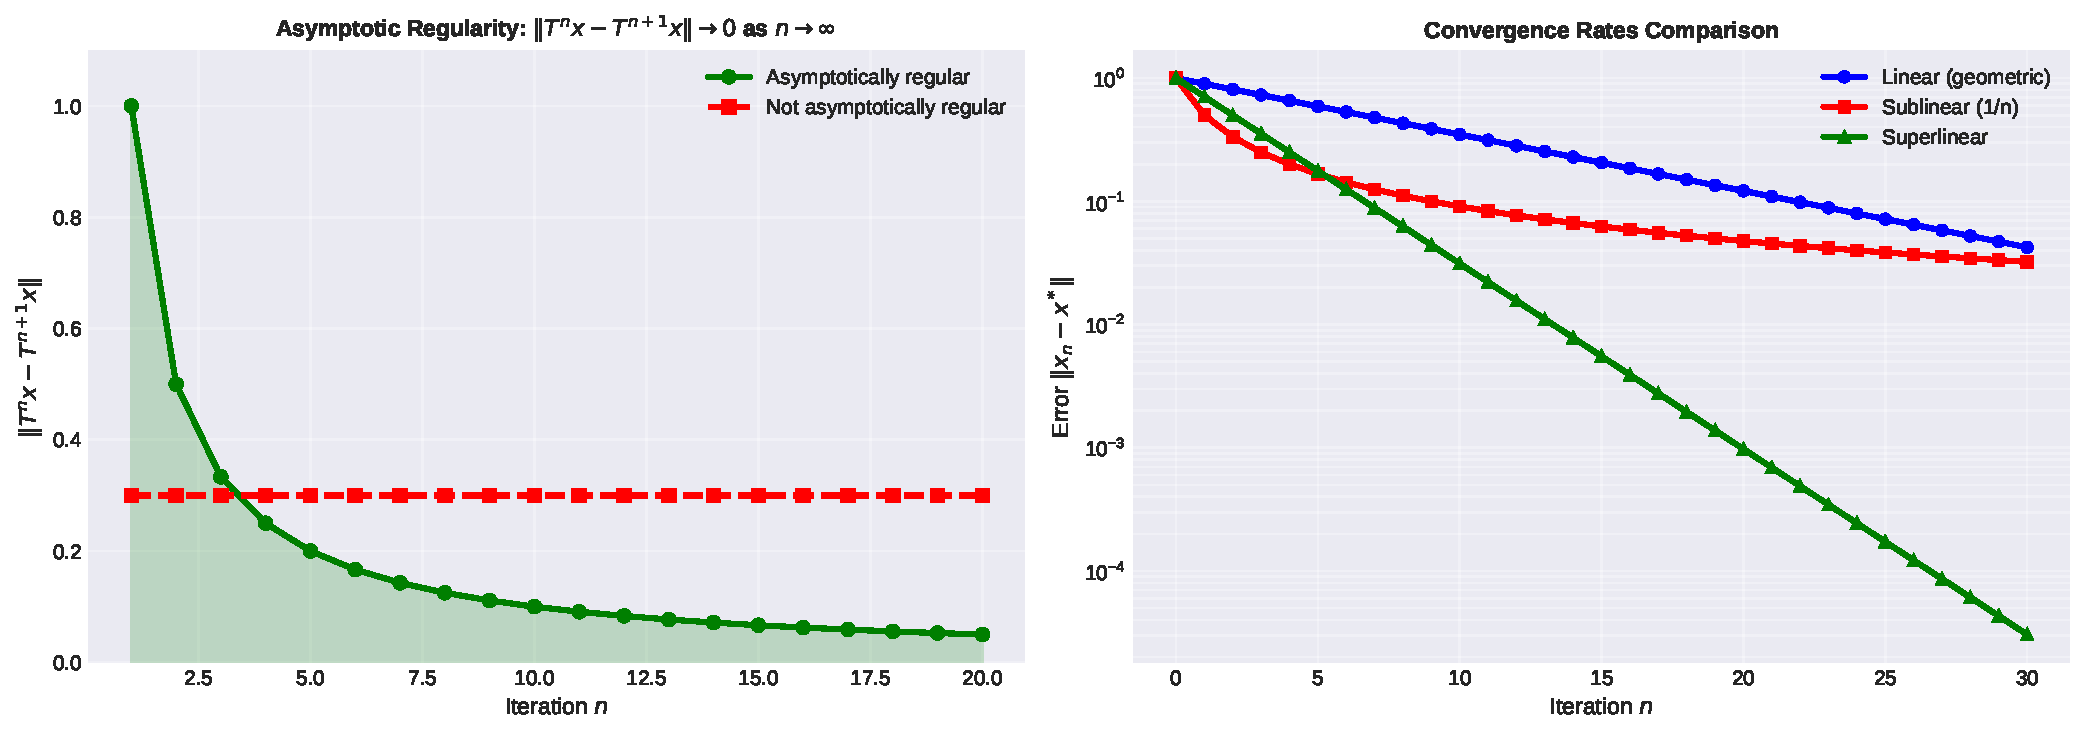
\includegraphics[width=0.95\textwidth]{asymptotic_regularity.pdf}
    \end{center}

    \begin{block}{Interpretation}
        \textbf{Left panel:} Asymptotic regularity requires iterates to become closer, with $\|T^n x - T^{n+1} x\| \to 0$.

        \textbf{Right panel:} Convergence rates vary dramatically:
        \begin{itemize}
            \item Linear (geometric): Fast, reliable
            \item Sublinear (1/n): Slow, guaranteed for asymptotic nonexpansive
            \item Superlinear: Very fast for special structures
        \end{itemize}
    \end{block}
\end{frame}

\begin{frame}[allowframebreaks]{Opial Condition Geometric Interpretation}
    \begin{center}
        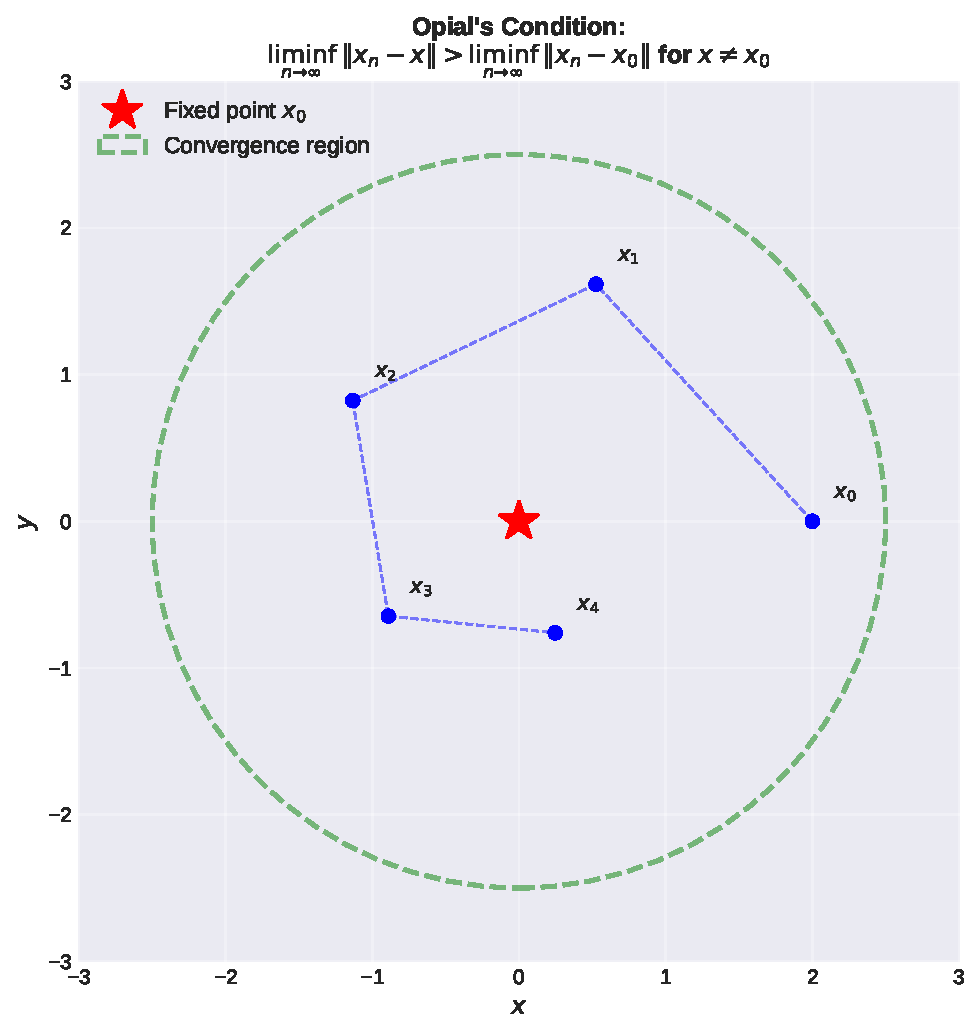
\includegraphics[width=0.95\textwidth]{opial_condition.pdf}
    \end{center}

    \begin{block}{What Opial's Condition Means}
        A weakly converging sequence $x_n \rightharpoonup x_0$ satisfies:
        \[\liminf \|x_n - x\| > \liminf \|x_n - x_0\| \quad \text{for all } x \neq x_0\]

        Geometrically: the weak limit $x_0$ is the ``nearest point'' in the limit-inferior sense.
    \end{block}

    \begin{block}{Importance}
        \begin{itemize}
            \item Ensures uniqueness of weak cluster points
            \item Fundamental for weak convergence theorems
            \item Holds automatically in Hilbert and $\ell_p$ spaces
        \end{itemize}
    \end{block}
\end{frame}

% ============================================================================
% SECTION 8: APPLICATIONS AND OPEN PROBLEMS
% ============================================================================
\section{Applications and Remarks}

\begin{frame}[allowframebreaks]{Applications of Fixed Point Theorems}
    \begin{block}{Differential and Integral Equations}
        Fixed point theorems provide existence proofs for solutions to:
        \begin{itemize}
            \item Ordinary differential equations: $x'(t) = f(t, x(t))$
            \item Integral equations: $x(t) = g(t) + \int_a^t K(t,s) x(s) ds$
            \item Functional equations
        \end{itemize}
    \end{block}

    \begin{block}{Optimization}
        \begin{itemize}
            \item Variational problems
            \item Saddle point problems
            \item Minimax theorems (related to fixed points)
        \end{itemize}
    \end{block}

    \begin{block}{Dynamical Systems}
        \begin{itemize}
            \item Periodic orbits of dynamical systems
            \item Bifurcation analysis
            \item Invariant manifolds
        \end{itemize}
    \end{block}

    \begin{block}{Numerical Analysis}
        \begin{itemize}
            \item Root finding via fixed point iteration
            \item Machine learning (fixed point methods in optimization)
            \item Control theory
        \end{itemize}
    \end{block}
\end{frame}

\begin{frame}[allowframebreaks]{Open Problems and Research Directions}
    \begin{block}{Known Open Questions}
        \begin{enumerate}
            \item Does every nonexpansive mapping on a bounded closed convex set have a fixed point in all Banach spaces?
            \item For which spaces does Opial's condition hold?
            \item Optimal convergence rates for different mapping classes
            \item Fixed point property for non-convex sets
        \end{enumerate}
    \end{block}

    \begin{block}{Current Research Trends}
        \begin{itemize}
            \item Multivalued mappings and set-valued analysis
            \item Fixed points in metric spaces and generalized metrics
            \item Applications to machine learning and optimization algorithms
            \item Variational inequalities and complementarity problems
            \item Fixed point theory for fractional operators
        \end{itemize}
    \end{block}
\end{frame}

\begin{frame}[allowframebreaks]{Remarks and Historical Context}
    \begin{block}{Historical Development}
        \begin{itemize}
            \item \textbf{1886}: Poincaré's ideas on fixed points in dynamics
            \item \textbf{1904}: Bohl's retraction argument
            \item \textbf{1910}: Brouwer's elegant proof for $\mathbb{B}^n$
            \item \textbf{1930}: Schauder extends to infinite dimensions
            \item \textbf{1950s-70s}: Systematic study of nonexpansive and asymptotically nonexpansive mappings
            \item \textbf{Modern era}: Applications to functional analysis, PDE, and optimization
        \end{itemize}
    \end{block}

    \begin{block}{Key Insights}
        \begin{itemize}
            \item Compactness and convexity are fundamental ingredients
            \item Topological degree and homology provide powerful tools
            \item Different spaces require adapted approaches
            \item Weak convergence methods extend classical results
        \end{itemize}
    \end{block}

    \begin{block}{Remark}
        Modern developments emphasize the interplay between topology, functional analysis, and computational methods in fixed point theory.
    \end{block}
\end{frame}

% ============================================================================
% CLOSING SLIDE
% ============================================================================
\begin{frame}[plain]
    \begin{center}
        \Large \textbf{Key Takeaways}

        \vspace{1cm}

        \begin{itemize}
            \item Fixed point theorems guarantee existence under specific conditions
            \item Brouwer: finite-dimensional; Schauder: compact maps
            \item Asymptotic nonexpansivity allows weaker convergence
            \item Opial's condition and asymptotic regularity are technical tools
            \item Applications span PDE, optimization, and dynamics
        \end{itemize}

        \vspace{1.5cm}

        \textit{``A fixed point is where the mapping rests; to find it is to understand the system.''}
    \end{center}
\end{frame}

\end{document}
